\let\negmedspace\undefined
\let\negthickspace\undefined
\documentclass[journal]{IEEEtran}
\usepackage[a5paper, margin=10mm, onecolumn]{geometry}
\usepackage{lmodern} % Ensure lmodern is loaded for pdflatex
\usepackage{tfrupee} % Include tfrupee package

\setlength{\headheight}{1cm} % Set the height of the header box
\setlength{\headsep}{0mm}     % Set the distance between the header box and the top of the text

\usepackage{gvv-book}
\usepackage{gvv}
\usepackage{cite}
\usepackage{amsmath,amssymb,amsfonts,amsthm}
\usepackage{algorithmic}
\usepackage{graphicx}
\usepackage{textcomp}
\usepackage{xcolor}
\usepackage{txfonts}
\usepackage{listings}
\usepackage{enumitem}
\usepackage{mathtools}
\usepackage{gensymb}
\usepackage{comment}
\usepackage[breaklinks=true]{hyperref}
\usepackage{tikz}
\usepackage{tkz-euclide} 
\usepackage{listings}
\def\inputGnumericTable{}                                 
\usepackage[latin1]{inputenc}                                
\usepackage{color}                                            
\usepackage{array}                                            
\usepackage{longtable}                                       
\usepackage{calc}                                             
\usepackage{multirow}                                         
\usepackage{hhline}                                           
\usepackage{ifthen}                                           
\usepackage{lscape}
\usetikzlibrary{matrix}

\begin{document}

\bibliographystyle{IEEEtran}
\vspace{3cm}

\title{10.3.3.1.3}
\author{EE24BTECH11002 - Agamjot Singh}
% \maketitle
% \newpage
% \bigskip
{\let\newpage\relax\maketitle}

\renewcommand{\thefigure}{\theenumi}
\renewcommand{\thetable}{\theenumi}
\setlength{\intextsep}{10pt} % Space between text and floats

\textbf{Question:}
\newline
Solve the following pair of linear equations,
\begin{align}
    3x - y = 3\\
    9x - 3y = 9
\end{align}
\textbf{Solution:}
\newline
Let
\begin{align}
    \vec{x} = \myvec{x\\y}
\end{align}
Expressing the system in matrix form,
\begin{align}
    \myvec{3 & -1\\9 & -3}\vec{x} = \myvec{3\\9}\\
    \text{which is of the form } A\vec{x} = \vec{b}
\end{align}
Any non-singular matrix $A$ can be expressed as a product of an upper triangular matrix $U$ and a lower triangular matrix $L$, such that
\begin{align}
    A &= LU\\
    \implies LU\vec{x} &= \vec{b}
\end{align}
$U$ is determined by row reducing $A$ using a pivot,
\begin{align}
    \myvec{3 & -1\\9 & -3} \xrightarrow{R_2 \to R_2 - 3R_1} \myvec{3 & -1\\0 & 0}
\end{align}
Let 
\begin{align}
    L = \myvec{1 & 0\\l & 1}
\end{align}
$l$ is the multiplier used to zero out $a_{21}$ in $A$.
\begin{align}
    L = \myvec{1 & 0\\3 & 1}
\end{align}
We see that there is a zero on the diagonal of the upper triangular matrix $U$ which implies that $A$ is singular and hence the system has either zero or infinitely many solutions.
\newline
Let $\vec{y} = U\vec{x}$,
\begin{align}
    L\vec{y} = \vec{b} \label{y_eq}
\end{align}
After we find $\vec{y}$, we find $\vec{x}$ using the following equation,
\begin{align}
    U\vec{x} = \vec{y} \label{x_eq}
\end{align}
Applying forward substitution on equation $\brak{\ref{y_eq}}$, we get,
\begin{align}
    \myvec{1 & 0\\3 & 1}\myvec{y_1\\y_2} &= \myvec{3\\9}\\
    \implies \myvec{y_1\\y_2} &= \myvec{3\\0}
\end{align}
Substituting $\vec{y}$ in equation $\brak{\ref{x_eq}}$, we get,
\begin{align}
    \myvec{3 & -1\\0 & 0} \myvec{x\\y} &= \myvec{3\\0}\\
    \implies 0\brak{x} + 0\brak{y} &= 0
\end{align}
This shows that the equation has infinitely many solutions.
\begin{figure}[h!]
  \centering
  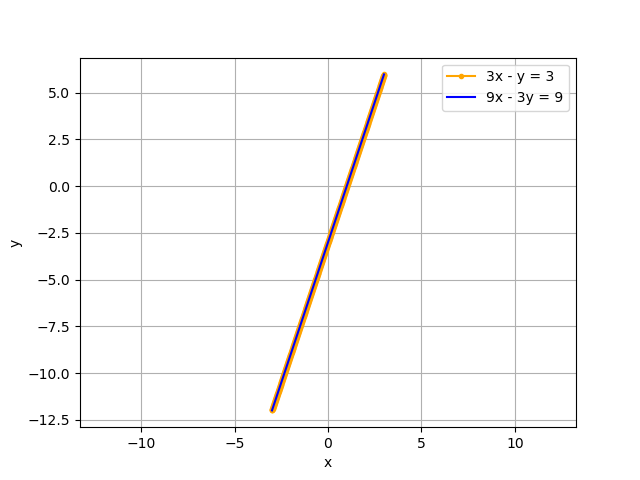
\includegraphics[width=0.7\columnwidth]{figs/graph.png}
  \caption{Plotting the two lines, which come out as parallel}
  \label{label}
\end{figure}

\end{document}
